\documentclass[amsmath,amssymb,aps,prl,onecolumn,notitlepage,superscriptaddress,longbibliography]{revtex4-2}
\usepackage{amsmath}
\usepackage{amssymb,dsfont,physics}
\usepackage{color}
\usepackage{tikz}
\usetikzlibrary{positioning}
\usetikzlibrary{automata,positioning}
\usetikzlibrary{fit,shapes.geometric}
\usetikzlibrary{decorations.pathmorphing}
\usetikzlibrary{arrows,matrix}
\usetikzlibrary{calc}
\usepackage{circuitikz}

\newcommand{\Sw}{\mathcal{S}}

\newcommand{\E}{\mathcal{E}}

\begin{document}

    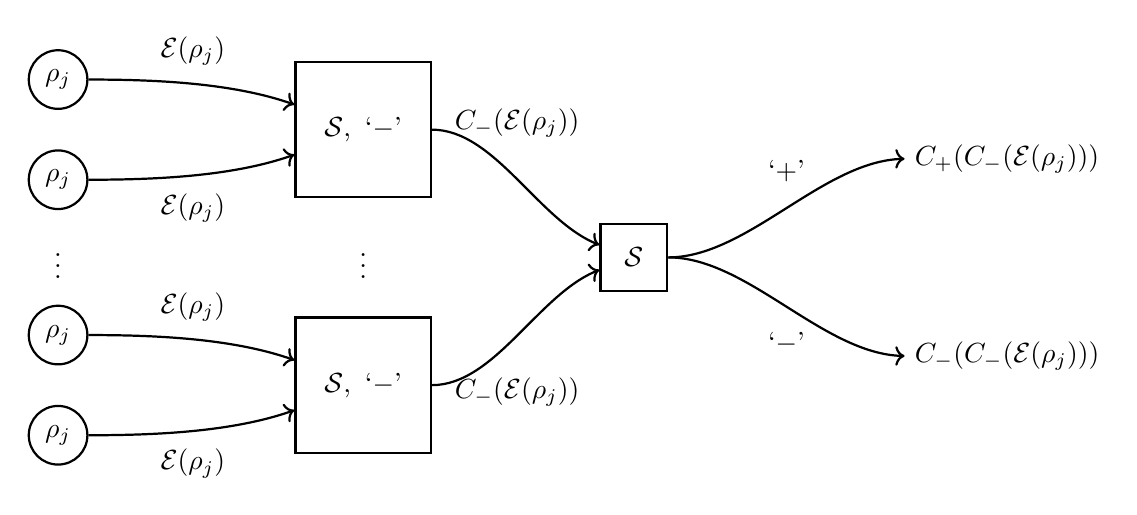
\begin{tikzpicture}[node distance={25mm}, thick,square/.style={regular polygon,regular polygon sides=4,minimum size=1.2cm}, main/.style={draw, circle,minimum size=0.5cm}]

    \node[main] (1) {$\rho_j$};
    \node[main] (2) [below=0.5cm of 1] {$\rho_j$};
    \coordinate(3) at ($(1)!0.5!(2)$);
    \node[square,draw] (4) [right=3cm of 3] {$\Sw$,\, `$-$'};
    \node[main] (5) [below=1.2cm of 2] {$\rho_j$};
    \node[main] (6) [below=0.5cm of 5] {$\rho_j$};
    \coordinate(7) at ($(5)!0.5!(6)$);
    \node[square,draw] (8) [right=3cm of 7] {$\Sw$,\, `$-$'};

    \coordinate(13) at ($(4)!0.5!(8)$);
    \node[square,draw] (14) [right=3cm of 13] {$\Sw$};
    \node[] (15)  at ($(4)!0.5!(8)$) {$\vdots$};
    \node[] (16)  at ($(2)!0.5!(5)$) {$\vdots$};
    \node[] (17) [above right= 0.5cm and 3cm of 14] {$C_{+}(C_{-} (\E(\rho_j)))$};
    \node[] (18) [below right= 0.5cm and 3cm of 14] {$C_{-}(C_{-} (\E(\rho_j)))$};

	\draw[->] (1) to [out=0,in=160,looseness=0.8] node[align=center,midway,above=0.1cm]{$\E(\rho_j)$} (4);
    \draw[->] (2) to [out=0,in=200,looseness=0.8] node[align=center,midway,below=0.1cm]{$\E(\rho_j)$} (4);
    \draw[->] (5) to [out=0,in=160,looseness=0.8] node[align=center,midway,above=0.1cm]{$\E(\rho_j)$} (8);
    \draw[->] (6) to [out=0,in=200,looseness=0.8] node[align=center,midway,below=0.1cm]{$\E(\rho_j)$} (8);
    \draw[->] (4) to [out=0,in=160,looseness=0.8] node[align=center,midway,above=0.4cm]{$C_{-} (\E(\rho_j))$} (14);
    \draw[->] (8) to [out=0,in=200,looseness=0.8] node[align=center,midway,below=0.4cm]{$C_{-} (\E(\rho_j))$} (14);
    \draw[->] (14) to [out=0,in=180,looseness=0.8] node[align=center,midway,above=0.2cm]{`$+$'} (17);
    \draw[->] (14) to [out=0,in=180,looseness=0.8] node[align=center,midway,below=0.2cm]{`$-$'} (18);
    \end{tikzpicture}

\end{document}